% !TEX root = ../diplomarbeit.tex
\clearpage
\section{Videoaufbereitung und Spielertracking}
\abschnittsautor{E. Akpinar}

\label{sec:Grundlage-Akpinar}

\enquote{Für die Auswertung von Laufwegen werden zeitlich zusammenhängende
Spielerpositionen in einem metrischen Koordinatensystem benötigt.
Der Teilbereich umfasst die Aufbereitung der Aufnahmen zweier
nebeneinander angeordneter Kameras, die Verfolgung erkannter Spieler
und die Abbildung ihrer Bildpositionen auf die Spielfeldebene.
Diese Verarbeitungsschritte verbinden die Objekterkennung mit den
Positionsdaten für die spätere Auswertung und Visualisierung.}~\cite{akpinar-codex-20261029a}

\subsection{Bildaufbereitung und Video-Stitching}
\enquote{Beim Video-Stitching werden die sich überlappenden Ansichten zweier Kameras
zu einer gemeinsamen Panoramaansicht zusammengefügt.}~\cite{akpinar-codex-20261029a}
Dazu werden übereinstimmende Punkte in beiden Kameraansichten, beispielsweise Schnittpunkte von Spielfeldlinien, einander zugeordnet. Anhand dieser Zuordnung werden die Bilder geometrisch ausgerichtet.
\enquote{Die Aufnahmen werden dazu auf eine gemeinsame Bildfläche transformiert.}~\cite{akpinar-codex-20261029a}
Die Open Computer Vision Library stellt dafür Verfahren zur Merkmalzuordnung, Bildtransformation, Belichtungsanpassung und Überblendung bereit~\cite{akpinar-opencv-stitching}.

Neben der räumlichen Ausrichtung müssen auch die Aufnahmezeitpunkte
übereinstimmen. Zeigt eine Kamera eine etwas spätere Spielsituation als die
andere, befindet sich ein laufender Spieler möglicherweise bereits an einer
anderen Stelle. Beim Zusammenfügen können dadurch doppelte oder versetzte
Spielerbilder entstehen. Für das Zwei-Kamera-System müssen die Aufnahmen
deshalb zeitlich aufeinander abgestimmt werden. Spielfeldlinien eignen sich
für die räumliche Ausrichtung, da sie während der Aufnahme an derselben
Stelle bleiben.

\subsection{Spielertracking über aufeinanderfolgende Bilder}
\abschnittsautor{E. Akpinar}

Die Objekterkennung bestimmt für jedes einzelne Bild, wo sich Spieler
befinden. Beim Tracking werden diese einzelnen Erkennungen über mehrere
Bilder hinweg miteinander verbunden. Das Ziel ist, denselben Spieler im
weiteren Verlauf wiederzuerkennen und seine Bewegung zu verfolgen.
Dazu erhält jede verfolgte Spur eine Kennnummer. Die Folge der zugeordneten
Positionen beschreibt die Bewegung des Spielers im Video. Die Verbindung
von Objekterkennung und anschließender zeitlicher Zuordnung wird als
\emph{Tracking-by-Detection} bezeichnet~\cite{akpinar-bewley-sort}.

Die zentrale Aufgabe des Trackings ist die Zuordnung zwischen bestehenden
Spuren und neu erkannten Spielern. Dabei geben die bisherige Position und
Bewegung Hinweise darauf, welche Erkennungen zusammengehören. Eine
Bewegungsvorhersage beschreibt, wo ein Spieler im nächsten Bild erwartet
wird. Der Vergleich dieser Vorhersage mit den neuen Erkennungen bildet
eine Grundlage für die weitere Zuordnung. Fehler in der Objekterkennung
wirken sich deshalb auch auf das Tracking aus: Wird ein Spieler übersehen
oder seine Position ungenau bestimmt, wird die Fortsetzung seiner Spur schwieriger~\cite{akpinar-bewley-sort}.

\subsection{Bildkoordinaten und die Ebene des Spielfelds}
Ein Videobild beschreibt eine Position durch eine Spalte und eine Zeile. Beide Werte werden in Pixeln angegeben. Der Ursprung des Bildes liegt links oben. Eine größere Zeilennummer bedeutet daher zunächst nur, dass der betreffende Punkt weiter unten im Bild erscheint. Im Feldplan wird dagegen die Entfernung auf dem Boden angegeben. Dort liegt der Ursprung des Versuchs vorne links. Die erste Koordinate wächst nach rechts, die zweite von der Kamera weg. Für die spätere Darstellung ist diese Festlegung ebenso wichtig wie die Einheit. Werden die Achsen vertauscht, kann ein gezeichneter Weg im Feld in die falsche Richtung zeigen, obwohl seine berechnete Länge gleich bleibt.

Die perspektivische Abbildung lässt sich am Hütchenraster erkennen. Die vordere und die hintere Reihe sind jeweils zehn Meter breit. Auf dem Bild nimmt die hintere Reihe jedoch nur einen Teil der Breite der vorderen ein. Ein einheitlicher Faktor in Metern pro Pixel würde entweder für den Vordergrund oder für den Hintergrund einen falschen Abstand liefern. Außerdem hängt die Änderung davon ab, in welcher Richtung ein Bildpunkt verschoben wird. Das ist für die Wahl des Messpunkts am Spieler entscheidend. Ein Fehler an der Unterkante eines Kastens kann in der Feldtiefe eine andere Wirkung haben als eine gleich große seitliche Verschiebung.

Die folgende Darstellung verwendet die gefundenen Hütchenpositionen im ersten Bild des Gehversuchs. Die Verbindungslinien dienen zur Orientierung zwischen benachbarten Hütchen. Sie sind keine im Video erkannten Feldlinien. Der Bildausschnitt ist auf das Raster begrenzt, während die Achsen weiterhin die Koordinaten des vollständigen Auswertungsbildes angeben.

Abb.~\ref{abb:em-persp} zeigt das Raster im Kamerabild des Gehversuchs.
\begin{figure}[htbp]\centering
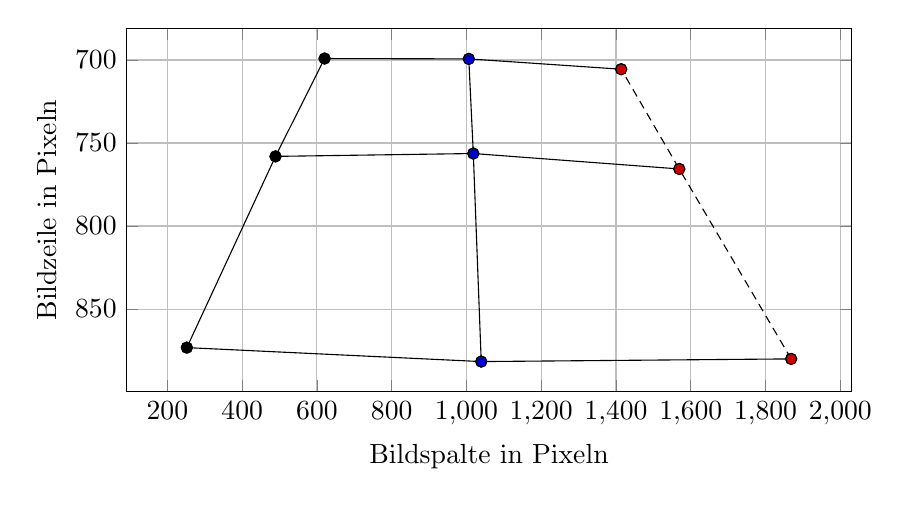
\begin{tikzpicture}\begin{axis}[width=.89\linewidth,height=6.2cm,grid=major,xlabel={Bildspalte in Pixeln},ylabel={Bildzeile in Pixeln},legend style={font=\small},legend pos=north west,y dir=reverse]
\addplot+[black,mark=*] coordinates {(251.987,873.201) (1039.484,881.611) (1868.562,880.001)};
\addplot+[black,mark=*] coordinates {(489.170,758.055) (1018.280,756.334) (1569.218,765.629)};
\addplot+[black,mark=*] coordinates {(620.463,699.135) (1006.213,699.349) (1413.856,705.567)};
\addplot+[black,mark=*] coordinates {(251.987,873.201) (489.170,758.055) (620.463,699.135)};
\addplot+[black,mark=*] coordinates {(1039.484,881.611) (1018.280,756.334) (1006.213,699.349)};
\addplot+[black,mark=*] coordinates {(1868.562,880.001) (1569.218,765.629) (1413.856,705.567)};
\end{axis}\end{tikzpicture}
\caption{das Raster im Kamerabild des Gehversuchs (eigene Darstellung)}\label{abb:em-persp}\end{figure}

\subsection{Berechnung der Feldkoordinaten durch eine Homographie}
Eine Homographie stellt eine Beziehung zwischen zwei Ebenen her. Für das Testfeld sind das die Abbildung des Bodens im Kamerabild und seine Darstellung in der Draufsicht. Die Rechnung verwendet eine Matrix mit drei Zeilen und drei Spalten. Zur üblichen Darstellung eines Bildpunkts $(u,v)$ kommt eine dritte Koordinate mit dem Wert eins hinzu. Die Multiplikation ergibt zunächst drei Hilfswerte~\cite{em-opencv-homographie}.
\[
\begin{pmatrix}a\\b\\w\end{pmatrix}
=H\begin{pmatrix}u\\v\\1\end{pmatrix},
\qquad X=a/w,\quad Y=b/w.
\]
Die Division durch $w$ erklärt, weshalb die Umrechnung vom Ort im Bild abhängt. Der Nenner enthält selbst die Bildkoordinaten. Zwei gleich lange Pfeile an verschiedenen Bildstellen können nach der Umrechnung unterschiedlich lang sein. Eine Multiplikation aller Matrixeinträge mit demselben Wert ändert dagegen das Ergebnis nicht, da sich der Faktor beim Dividieren kürzt. Vier passende Punktpaare in allgemeiner Lage reichen zur Bestimmung der acht unabhängigen Parameter aus~\cite{em-opencv-homographie}.

Für jeden verwendeten Bodenpunkt muss feststehen, welcher Feldmarkierung er entspricht. Eine vertauschte Ecke ist besonders leicht zu übersehen, wenn nur die vier eingegebenen Punkte erneut durchgerechnet werden. Die Matrix wird gerade so bestimmt, dass sie diese Zuordnungen erfüllt. Eine kleine Abweichung an diesen vier Stellen sagt daher wenig über die Lage eines Spielers im Inneren des Feldes aus.

Auch bei korrekter Zuordnung gilt die Abbildung für die vereinbarte Ebene. Ein aufrechter Spieler reicht über diese Ebene hinaus. Wird beispielsweise sein Kopf in die Formel eingesetzt, entsteht zwar ein Zahlenpaar. Es beschreibt jedoch den Schnitt der entsprechenden Sichtlinie mit der Bodenebene. Als Näherung für seinen Standort ist deshalb ein Punkt in der Nähe des Bodenkontakts erforderlich.

\subsection{Unabhängige Kontrolle und örtliche Empfindlichkeit}
Eine Kontrolle beantwortet zwei verschiedene Fragen. Bei der ersten wird ein einzelner bekannter Feldpunkt geprüft. Dazu wird sein Bildpunkt umgerechnet und mit seinen gemessenen Feldkoordinaten verglichen. Die Länge des Unterschiedsvektors ist der Positionsfehler dieses Punkts. Bei der zweiten Frage wird der Abstand zwischen zwei umgerechneten Punkten geprüft. Dieser Vergleich ist für die Laufwegauswertung besonders anschaulich. Beide Punkte können beispielsweise um denselben Betrag nach rechts versetzt sein. Ihr Abstand bleibt in diesem Fall richtig, obwohl ihre absoluten Positionen falsch sind.

Als Rechenbeispiel dient das hintere mittlere Hütchen des gespeicherten Referenzprofils. Sein Sollpunkt liegt bei $(5;10)$ Metern. Die vier Ecken liefern für den angeklickten Bildpunkt näherungsweise $(4{,}83;10{,}35)$ Meter. Damit liegt die berechnete Position rund 17 Zentimeter weiter links und 35 Zentimeter weiter hinten. Aus beiden Anteilen ergibt sich ein Abstand von etwa 39 Zentimetern zum Sollpunkt. Die Richtung geht verloren, wenn ausschließlich dieser letzte Zahlenwert angegeben wird.

Eine zweite Untersuchung hält die Matrix fest und verschiebt nur den auszuwertenden Bildpunkt. Die Werte in der Tabelle stammen aus der gespeicherten Sichtprüfung vom 13. November. Sie geben die Änderung des berechneten Orts bei genau einem Pixel Verschiebung an. Die Messung enthält weder die Unsicherheit des Maßbands noch Änderungen der vier zur Kalibrierung verwendeten Ecken. Sie eignet sich daher zur Beurteilung der Bildauswahl, aber nicht zur Angabe eines allgemeinen Fehlerintervalls.

Siehe Tab.~\ref{tab:em-pixel}.
\begin{table}[htbp]\centering\caption{Wirkung eines Pixels im Referenzbild, in Zentimetern (eigene Sichtprüfung)}\label{tab:em-pixel}
\begin{tabular}{@{}llll@{}}\toprule Hütchen & nach rechts & nach oben & nach unten\\\midrule
hinten links & 1,2 & 12,0 & 11,9\\
hinten rechts & 1,3 & 12,4 & 12,3\\
vorne rechts & 0,6 & 3,3 & 3,3\\
vorne links & 0,6 & 3,1 & 3,0\\
hinten mitte & 1,3 & 12,2 & 12,1\\
mitte links & 0,9 & 6,6 & 6,6\\
mitte mitte & 1,0 & 6,7 & 6,7\\
mitte rechts & 1,0 & 7,0 & 6,9\\
vorne mitte & 0,6 & 2,7 & 2,7\\\bottomrule\end{tabular}\end{table}


\subsection{Einfluss der Bewegungsrichtung auf den Wegfehler}
Die bisher betrachtete Abweichung eines einzelnen Feldpunkts lässt sich nicht unmittelbar auf einen ganzen Lauf übertragen. Werden alle Positionen eines Läufers um denselben Vektor verschoben, verläuft die Spur im Feld zwar an der falschen Stelle, die Abstände aufeinanderfolgender Punkte bleiben aber gleich. Anders verhält es sich, wenn sich der Fehler mit dem Ort ändert. Bei einem Lauf in die Feldtiefe können Start und Ziel unterschiedlich stark versetzt sein. Die berechnete Strecke kann dadurch je nach Richtung länger oder kürzer ausfallen.

Im Referenzprofil liegen für fünf unabhängige Punkte sowohl die erwarteten als auch die umgerechneten Koordinaten vor. Für jeden Punkt lässt sich ausrechnen, wie groß die Abweichung entlang der X-Achse und entlang der Y-Achse ist. Die folgende Darstellung verwendet diese Differenzen in Zentimetern. Ein positiver Wert in der zweiten Richtung bedeutet bei der gewählten Orientierung eine Verschiebung nach hinten. Der Nullpunkt des Diagramms entspricht einer exakt getroffenen Feldposition, nicht einer bestimmten Stelle des Testfeldes.

Abb.~\ref{abb:em-richtung} zeigt die Komponenten der Abweichung im verwendeten Referenzprofil.
\begin{figure}[htbp]\centering
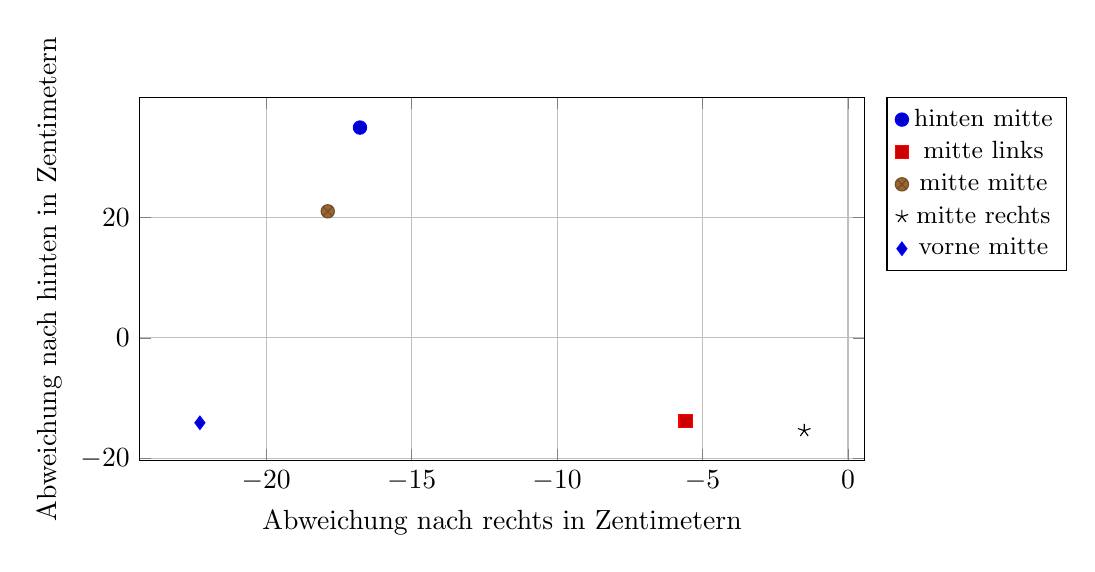
\begin{tikzpicture}\begin{axis}[width=.89\linewidth,height=6.2cm,grid=major,xlabel={Abweichung nach rechts in Zentimetern},ylabel={Abweichung nach hinten in Zentimetern},legend style={font=\small},legend pos=north west,legend pos=outer north east]
\addplot+[only marks,mark size=2.4pt] coordinates {(-16.777,34.891)};
\addlegendentry{hinten mitte}
\addplot+[only marks,mark size=2.4pt] coordinates {(-5.580,-13.760)};
\addlegendentry{mitte links}
\addplot+[only marks,mark size=2.4pt] coordinates {(-17.885,20.992)};
\addlegendentry{mitte mitte}
\addplot+[only marks,mark size=2.4pt] coordinates {(-1.503,-15.399)};
\addlegendentry{mitte rechts}
\addplot+[only marks,mark size=2.4pt] coordinates {(-22.280,-14.104)};
\addlegendentry{vorne mitte}
\end{axis}\end{tikzpicture}
\caption{die Komponenten der Abweichung im verwendeten Referenzprofil (eigene Darstellung)}\label{abb:em-richtung}\end{figure}
Die fünf Punkte stellen verschiedene Orte derselben Referenz dar. Ihr Mittelwert wäre für die Beurteilung einer einzelnen Laufrichtung wenig aussagekräftig, weil sich positive und negative Anteile gegenseitig aufheben können. Für eine Überprüfung außerhalb der neun bekannten Hütchen wäre eine zusätzliche vermessene Bodenmarkierung geeignet. Sie müsste bereits vor der Auswertung festgelegt werden. Eine nachträgliche Auswahl gerade jener Stelle, an der das Ergebnis besonders gut passt, würde die Aussagekraft des Vergleichs einschränken.

\subsection{Zeitliche Abtastung und Länge einer Bewegungsspur}
Zur Beschreibung eines Weges gehören neben den Positionen ihre Aufnahmezeitpunkte. Liegen zwei Positionen eines Spielers vor, ist zunächst nur der Abstand ihrer Endpunkte bekannt. Für eine Folge von gültigen Feldpositionen $P_i=(X_i,Y_i)$ ergibt sich der beobachtete Weg eines zusammenhängenden Abschnitts als Summe
\[
s=\sum_{i=1}^{n}\sqrt{(X_i-X_{i-1})^2+(Y_i-Y_{i-1})^2}.
\]
Start- und Endpunkt allein reichen bei gekrümmten Wegen nicht aus. Beim Kreislaufen können beide dicht beieinander liegen, obwohl eine längere Strecke zurückgelegt wurde. Auch zwischen zwei aufeinanderfolgenden Messungen ersetzt die Rechnung die Bewegung durch eine gerade Verbindung. Bei einer engen Kurve kann diese Verbindung den tatsächlich zurückgelegten Bogen verkürzen.

Ein zweiter Einfluss wirkt in die andere Richtung. Ändert sich bei einer stehenden Person der erkannte Kasten geringfügig, wandert der abgeleitete Bodenpunkt. Jeder dieser kleinen Abstände geht mit positivem Vorzeichen in die Summe ein. Ein Ausschlag nach rechts und die Rückkehr nach links heben einander bei der Streckenberechnung nicht auf. Die Verbindung zwischen erstem und letztem Punkt kann dabei sehr kurz bleiben. Bei der Bewertung eines Verfahrens sind somit sowohl ruhige Phasen als auch Richtungswechsel von Interesse.

Das folgende geometrische Beispiel verwendet drei bekannte Punkte und dient ausschließlich zur Erklärung der Rechnung. Der mittlere Punkt liegt einen Meter neben der geraden Verbindung. Bei einer Auswertung nur des ersten und letzten Punkts geht die Richtungsänderung vollständig verloren.

Abb.~\ref{abb:em-bogen} zeigt den Einfluss eines Zwischenpunkts auf die Weglänge.
\begin{figure}[htbp]\centering
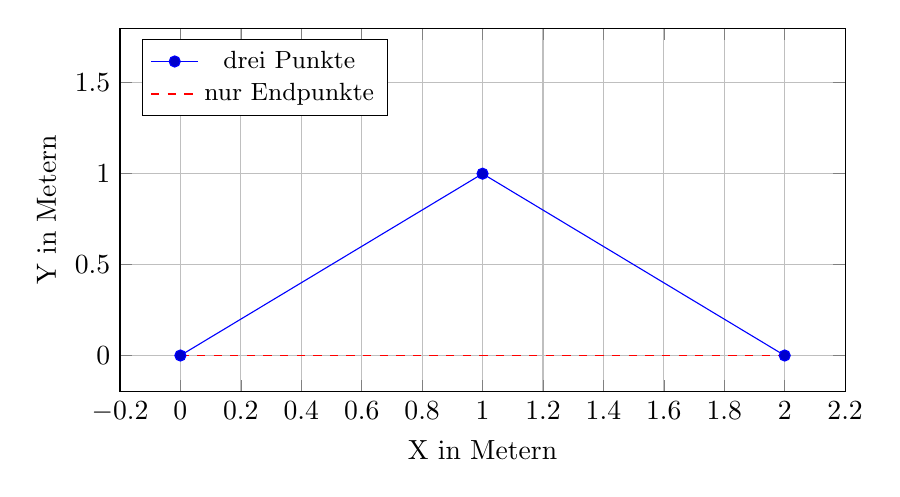
\begin{tikzpicture}\begin{axis}[width=.89\linewidth,height=6.2cm,grid=major,xlabel={X in Metern},ylabel={Y in Metern},legend style={font=\small},legend pos=north west,ymin=-0.2,ymax=1.8]
\addplot+[mark=*] coordinates {(0.000,0.000) (1.000,1.000) (2.000,0.000)};
\addlegendentry{drei Punkte}
\addplot+[dashed,mark=none] coordinates {(0.000,0.000) (2.000,0.000)};
\addlegendentry{nur Endpunkte}
\end{axis}\end{tikzpicture}
\caption{den Einfluss eines Zwischenpunkts auf die Weglänge (eigene Darstellung)}\label{abb:em-bogen}\end{figure}
Die direkte Verbindung beträgt zwei Meter. Mit dem Zwischenpunkt ergeben sich zwei gleich lange Teilstrecken von jeweils $\sqrt{2}$ Metern, zusammen rund 2,83 Meter. Für die Interpretation eines realen Videos muss zusätzlich geklärt werden, ob die seitliche Bewegung tatsächlich stattgefunden hat oder ob sie aus einer ungenauen Positionsbestimmung stammt.

\subsection{Beobachtung, Zuordnung und fehlende Messwerte}
Bei einer Begegnung zweier Spieler kann die Feldzuordnung für das ganze Bild gültig sein, obwohl nur einer der beiden Bodenpunkte sichtbar ist. Für einen Weg sind daher drei Entscheidungen zu unterscheiden. Zuerst muss eine Person im Bild gefunden werden. Anschließend muss der Kasten der richtigen Spur angehören. Schließlich muss sein unterer Rand eine brauchbare Aussage über die Position am Boden erlauben. Der Ausfall einer Entscheidung kann einen gültigen Wert für eine andere Person im selben Bild unberührt lassen.

Das zeigt sich besonders bei einer kurzen Verdeckung. Vor dem Hindernis ist die Person an einer bestimmten Stelle sichtbar und nach dem Hindernis an einer anderen. Selbst wenn beide Kästen sicher zur selben Person gehören, bleibt der genaue Weg dazwischen unbekannt. Aus den Endpunkten lässt sich eine geradlinige Schätzung ableiten. Ein Ausweichschritt oder ein Richtungswechsel hinter der anderen Person ist darin nicht enthalten. Fehlt auch die sichere Zuordnung nach der Begegnung, würde dieselbe Rechnung möglicherweise die Wege zweier verschiedener Personen verbinden.

Für die spätere Bewertung werden daher die erfasste Zeit, die beobachtete Strecke und eine gegebenenfalls geschätzte Strecke getrennt betrachtet. Eine Laufwegangabe erhält erst zusammen mit diesen Angaben eine eindeutige Bedeutung. Besonders bei kurzen Testvideos kann bereits eine einzige fehlende Sekunde einen erheblichen Anteil des Versuchs betreffen.
\clearpage
